% Options for packages loaded elsewhere
\PassOptionsToPackage{unicode}{hyperref}
\PassOptionsToPackage{hyphens}{url}
\PassOptionsToPackage{dvipsnames,svgnames,x11names}{xcolor}
%
\documentclass[
  a4paper,
  12pt]{article}

\usepackage{amsmath,amssymb}
\usepackage{iftex}
\ifPDFTeX
  \usepackage[T1]{fontenc}
  \usepackage[utf8]{inputenc}
  \usepackage{textcomp} % provide euro and other symbols
\else % if luatex or xetex
  \usepackage{unicode-math}
  \defaultfontfeatures{Scale=MatchLowercase}
  \defaultfontfeatures[\rmfamily]{Ligatures=TeX,Scale=1}
\fi
\usepackage{lmodern}
\ifPDFTeX\else  
    % xetex/luatex font selection
\fi
% Use upquote if available, for straight quotes in verbatim environments
\IfFileExists{upquote.sty}{\usepackage{upquote}}{}
\IfFileExists{microtype.sty}{% use microtype if available
  \usepackage[]{microtype}
  \UseMicrotypeSet[protrusion]{basicmath} % disable protrusion for tt fonts
}{}
\makeatletter
\@ifundefined{KOMAClassName}{% if non-KOMA class
  \IfFileExists{parskip.sty}{%
    \usepackage{parskip}
  }{% else
    \setlength{\parindent}{0pt}
    \setlength{\parskip}{6pt plus 2pt minus 1pt}}
}{% if KOMA class
  \KOMAoptions{parskip=half}}
\makeatother
\usepackage{xcolor}
\usepackage[left=2.5cm, right=2.5cm, top=3cm, bottom=3cm]{geometry}
\setlength{\emergencystretch}{3em} % prevent overfull lines
\setcounter{secnumdepth}{2}
% Make \paragraph and \subparagraph free-standing
\ifx\paragraph\undefined\else
  \let\oldparagraph\paragraph
  \renewcommand{\paragraph}[1]{\oldparagraph{#1}\mbox{}}
\fi
\ifx\subparagraph\undefined\else
  \let\oldsubparagraph\subparagraph
  \renewcommand{\subparagraph}[1]{\oldsubparagraph{#1}\mbox{}}
\fi


\providecommand{\tightlist}{%
  \setlength{\itemsep}{0pt}\setlength{\parskip}{0pt}}\usepackage{longtable,booktabs,array}
\usepackage{calc} % for calculating minipage widths
% Correct order of tables after \paragraph or \subparagraph
\usepackage{etoolbox}
\makeatletter
\patchcmd\longtable{\par}{\if@noskipsec\mbox{}\fi\par}{}{}
\makeatother
% Allow footnotes in longtable head/foot
\IfFileExists{footnotehyper.sty}{\usepackage{footnotehyper}}{\usepackage{footnote}}
\makesavenoteenv{longtable}
\usepackage{graphicx}
\makeatletter
\def\maxwidth{\ifdim\Gin@nat@width>\linewidth\linewidth\else\Gin@nat@width\fi}
\def\maxheight{\ifdim\Gin@nat@height>\textheight\textheight\else\Gin@nat@height\fi}
\makeatother
% Scale images if necessary, so that they will not overflow the page
% margins by default, and it is still possible to overwrite the defaults
% using explicit options in \includegraphics[width, height, ...]{}
\setkeys{Gin}{width=\maxwidth,height=\maxheight,keepaspectratio}
% Set default figure placement to htbp
\makeatletter
\def\fps@figure{htbp}
\makeatother
% definitions for citeproc citations
\NewDocumentCommand\citeproctext{}{}
\NewDocumentCommand\citeproc{mm}{%
  \begingroup\def\citeproctext{#2}\cite{#1}\endgroup}
\makeatletter
 % allow citations to break across lines
 \let\@cite@ofmt\@firstofone
 % avoid brackets around text for \cite:
 \def\@biblabel#1{}
 \def\@cite#1#2{{#1\if@tempswa , #2\fi}}
\makeatother
\newlength{\cslhangindent}
\setlength{\cslhangindent}{1.5em}
\newlength{\csllabelwidth}
\setlength{\csllabelwidth}{3em}
\newenvironment{CSLReferences}[2] % #1 hanging-indent, #2 entry-spacing
 {\begin{list}{}{%
  \setlength{\itemindent}{0pt}
  \setlength{\leftmargin}{0pt}
  \setlength{\parsep}{0pt}
  % turn on hanging indent if param 1 is 1
  \ifodd #1
   \setlength{\leftmargin}{\cslhangindent}
   \setlength{\itemindent}{-1\cslhangindent}
  \fi
  % set entry spacing
  \setlength{\itemsep}{#2\baselineskip}}}
 {\end{list}}
\usepackage{calc}
\newcommand{\CSLBlock}[1]{\hfill\break\parbox[t]{\linewidth}{\strut\ignorespaces#1\strut}}
\newcommand{\CSLLeftMargin}[1]{\parbox[t]{\csllabelwidth}{\strut#1\strut}}
\newcommand{\CSLRightInline}[1]{\parbox[t]{\linewidth - \csllabelwidth}{\strut#1\strut}}
\newcommand{\CSLIndent}[1]{\hspace{\cslhangindent}#1}

\usepackage{setspace}\doublespacing
\makeatletter
\@ifpackageloaded{caption}{}{\usepackage{caption}}
\AtBeginDocument{%
\ifdefined\contentsname
  \renewcommand*\contentsname{Table of contents}
\else
  \newcommand\contentsname{Table of contents}
\fi
\ifdefined\listfigurename
  \renewcommand*\listfigurename{List of Figures}
\else
  \newcommand\listfigurename{List of Figures}
\fi
\ifdefined\listtablename
  \renewcommand*\listtablename{List of Tables}
\else
  \newcommand\listtablename{List of Tables}
\fi
\ifdefined\figurename
  \renewcommand*\figurename{Figure}
\else
  \newcommand\figurename{Figure}
\fi
\ifdefined\tablename
  \renewcommand*\tablename{Table}
\else
  \newcommand\tablename{Table}
\fi
}
\@ifpackageloaded{float}{}{\usepackage{float}}
\floatstyle{ruled}
\@ifundefined{c@chapter}{\newfloat{codelisting}{h}{lop}}{\newfloat{codelisting}{h}{lop}[chapter]}
\floatname{codelisting}{Listing}
\newcommand*\listoflistings{\listof{codelisting}{List of Listings}}
\makeatother
\makeatletter
\makeatother
\makeatletter
\@ifpackageloaded{caption}{}{\usepackage{caption}}
\@ifpackageloaded{subcaption}{}{\usepackage{subcaption}}
\makeatother
\ifLuaTeX
  \usepackage{selnolig}  % disable illegal ligatures
\fi
\usepackage{bookmark}

\IfFileExists{xurl.sty}{\usepackage{xurl}}{} % add URL line breaks if available
\urlstyle{same} % disable monospaced font for URLs
\hypersetup{
  pdftitle={Developing Multivariate Proximity-based Spatial Autocorrelation Statistics Using Random Forests},
  pdfauthor={Woohyung Kim},
  pdfkeywords={keyword1, keyword2, keyword3},
  colorlinks=true,
  linkcolor={blue},
  filecolor={Maroon},
  citecolor={Blue},
  urlcolor={Blue},
  pdfcreator={LaTeX via pandoc}}

\title{Developing Multivariate Proximity-based Spatial Autocorrelation
Statistics Using Random Forests}
\author{Woohyung Kim}
\date{}

\begin{document}
\maketitle
\begin{abstract}
Abstract Here
\end{abstract}

\section{Introduction}\label{introduction}

\section{Literature Review}\label{literature-review}

Early spatial statistics introduced measures to quantify global spatial
autocorrelation---the overall degree to which values of a variable are
similar or dissimilar at nearby locations. The two classic indices are
Moran's \emph{I} (\citeproc{ref-moran1950}{Moran 1950}), a spatial
analog of a correlation coefficient, and Geary's \emph{c}
(\citeproc{ref-geary1954}{Geary 1954}), which is based on squared
differences between neighboring values. A major limitation of these
global measures is that they can mask local patterns by averaging over
spatial heterogeneity. This motivated the development of local
statistics, most notably the Local Indicators of Spatial Association
(LISA) framework by Anselin (\citeproc{ref-anselin1995}{1995}), which
decomposed global statistics into their local counterparts to identify
\emph{where} significant clustering or outlier patterns occur.

Building on this foundation, subsequent research has extended these
concepts to a multivariate context. Wartenberg
(\citeproc{ref-wartenberg1985}{1985}) pioneered this effort by
integrating principal component analysis with spatial autocorrelation.
This was followed by the development of bivariate measures like Lee's
\emph{L} (\citeproc{ref-lee2001}{S.-I. Lee 2001}) and, more recently,
local multivariate statistics such as the Mahalanobis distance-based
measure (\citeproc{ref-lee2012}{M. Lee 2012}) and the multivariate Local
Geary's \emph{c} (\citeproc{ref-anselin2019}{Anselin 2019}). These
studies established important frameworks for analyzing spatial patterns
across multiple variables simultaneously.

However, these traditional and even more recent multivariate spatial
statistics face fundamental challenges. First, they are often limited by
assumptions of linearity or specific data distributions, restricting
their ability to capture complex, non-linear interactions. Second, these
challenges are compounded in high-dimensional datasets. Foundational
work by Beyer et al. (\citeproc{ref-beyer1999}{1999}) demonstrated that
as dimensionality increases, the contrast between the farthest and
nearest data points to a query point vanishes---a phenomenon known as
distance concentration. This makes the very concept of a `nearest
neighbor' unstable and qualitatively meaningless. Furthermore, Aggarwal
et al. (\citeproc{ref-aggarwal2001}{2001}) showed that this problem is
sensitive to the choice of distance metric, with the commonly used
Euclidean distance (L2 norm) losing contrast more rapidly than other
metrics. Third, handling mixed data types is often not straightforward.
While methods like join-count statistics exist for categorical data,
they are typically limited to binary or low-cardinality setting, and
addressing datasets with both continuous and categorical variables
requires complex pre-processing. Crucially, even advanced framework like
Lee's \emph{L} (\citeproc{ref-lee2001}{S.-I. Lee 2001}), the Mahalanobis
distance-based statistics (\citeproc{ref-lee2012}{M. Lee 2012}), and the
multivariate Local Geary's \emph{c} (\citeproc{ref-anselin2019}{Anselin
2019}) are not immune to these limitations, as they rely on linear
assumptions or distance metrics susceptible to high-dimensional
instability.

The measurement of spatial autocorrelation is fundamentally an
unsupervised learning problem, as it seeks to identify spatial patterns
within a set of attributes without a predefined dependent variable. To
address the aforementioned limitations of traditional approaches, this
study turns to a powerful, data-adaptive similarity measure from machine
learning: the Random Forest (RF) proximity
(\citeproc{ref-breiman2001}{Breiman 2001}). This technique, particularly
in its unsupervised mode known as Unsupervised Random Forest (URF),
operates on the core assumption that if data contains inherent
structure, it can be distinguished from a randomly generated counterpart
(\citeproc{ref-shi2006}{Shi and Horvath 2006}). The effectiveness of
this URF-based proximity is well-documented across diverse fields. It
has been widely used for outlier and anomaly detection, such as
identifying network intrusions (\citeproc{ref-zhang2008}{Zhang et al.
2008}) and defective semiconductor chips (\citeproc{ref-wu2007}{Wu et
al. 2007}). In clustering and visualization, URF has proven superior to
traditional distance metrics for interpreting high-dimensional
biological data and has been used for data cleaning by identifying
duplicate records (\citeproc{ref-omar2022}{Omar et al. 2022}).
Particularly relevant to this study, URF proximity has shown significant
potential in spatial analysis. Peerbhay et al.
(\citeproc{ref-peerbhay2015}{2015}) and Peerbhay et al.
(\citeproc{ref-peerbhay2016}{2016}) demonstrated this by analyzing
aerial hyperspectral imagery to detect invasive plant species. By
extracting outlier scores from the proximity matrix and combining them
with spatial anomaly detection techniques, they successfully mapped
plant clusters without pre-existing labels, providing crucial evidence
that RF proximity can effectively capture subtle similarities to
identify spatial patterns.

The literature thus validates URF proximity as a robust method for
uncovering hidden structures in complex data. However, the formalization
of this powerful, assumption-free similarity measure into a new
statistic for quantifying multivariate spatial autocorrelation remains a
largely unexplored research gap. This study aims to fill this gap in
spatial statistics by leveraging the proven effectiveness of URF
proximity---specifically an advanced implementation called Path
Proximity (\citeproc{ref-kruber2019}{Kruber et al. 2019}), which
measures similarity based on the entire decision path through a
tree---as the core engine for measuring attribute similarity. By
integrating this measure into a spatial autocorrelation framework, we
develop a new statistic capable of handling multivariate, non-linear
rxelationships and mixed data types in a single, unified measure.

\section{Multivariate Proximity-based Spatial Autocorrelation Statistics
(MPSA)}\label{multivariate-proximity-based-spatial-autocorrelation-statistics-mpsa}

This section introduces the Multivariate Proximity-based Spatial
Autocorrelation Statistic (MPSA), a novel measure designed to quantify
the degree of spatial autocorrelation in multivariate data. MPSA
integrates a proximity matrix that captures the attribute similarity
between observational units with a spatial weights matrix that
represents spatial adjacency, enabling a quantitative assessment of the
extent to which similar attribute patterns are spatially clustered.

\subsection{Unsupervised Random Forest and the Construction of Proximity
Matrix}\label{unsupervised-random-forest-and-the-construction-of-proximity-matrix}

The proximity is computed using an unsupervised random forests(URF). To
implement the URF, a synthetic dataset \(\mathbf{X_{\text{fake}}}\) is
first generated to be contrasted with the original data matrix
\(\mathbf{X}\). There are two common approaches to generate such
synthetic data (\citeproc{ref-breiman2003}{Breiman 2003}). In the
\emph{Addcl1} approach, synthetic samples are drawn independently from
the marginal distributions of each variable in the observed data,
thereby preserving individual variable distributions while removing
inter-variable dependence. In contrast, \emph{Addcl2} samples are drawn
from uniformly from a hyper-rectangular space defined by the range of
each variable in the original data, which alters both the distributional
shape and the underlying correlation structure. According to Shi and
Horvath (\citeproc{ref-shi2006}{2006}), the \emph{Addcl1} method tends
to outperform \emph{Addcl2} in practical applications. Consequently,
this study adopts \emph{Addcl1} for the main analysis.

This approach fundamentally differs from traditional distance-based
methods that are susceptible to the curse of dimensionality. Whereas
geometric metrics compute distance across all dimensions simultaneously,
URF builds its similarity measure from a series of decision trees. Each
split in a tree is determined by evaluating only a small, random subset
of variables, thereby mitigating the influence of noisy, irrelevant
dimensions. As a result, the resulting proximity score reflects a
structural similarity---how often two observations follow similar
decision paths---rather than a direct geometric distance, making it
robust in high-dimensional space.

After the URF classifier trained, the proximity between observations is
calculated. The standard approach computes proximity as the proportion
of trees in which two observations fall into the same terminal node. A
critical limitation of this method, however, is its high sensitivity to
the tree pruning process (\citeproc{ref-kruber2019}{Kruber et al.
2019}). The degree of pruning directly determines the number of terminal
nodes; aggressive pruning may oversimplify the data structure, while
minimal pruning often leads to a highly sparse matrix where most
observation pairs receive a zero value. This instability makes it
difficult to obtain a robust similarity measure.

To overcome this challenge, this study employs Path Proximity, a more
robust measure of similarity proposed by Kruber et al.
(\citeproc{ref-kruber2019}{2019}). This technique considers the full
paths of data points through the trees, not just the terminal nodes. The
path for an observation \(i\) in a tree \(t\) is defined as the set of
nodes it passes through \(\mathcal{T}_{i, t}\). To compare the paths of
two observations, \(i\) and \(j\), this technique uses the Jaccard
Index, which measures the similarity between their path sets. The final
Path Proximity is the average of these Jaccard indices over all \(T\)
trees in the forest, formulated as:
\begin{equation}\phantomsection\label{eq-path-proximity-jaccard}{
\mathbf{P}_{ij} = \frac{1}{T} \sum_{t=1}^{T} \frac{|\mathcal{T}_{i,t} \cap \mathcal{T}_{j,t}|}{|\mathcal{T}_{i,t} \cup \mathcal{T}_{j,t}|} = \frac{1}{T} \sum_{t=1}^{T} \frac{|\mathcal{T}_{i,t} \cap \mathcal{T}_{j,t}|}{|\mathcal{T}_{i,t}| + |\mathcal{T}_{j,t}| - |\mathcal{T}_{i,t} \cap \mathcal{T}_{j,t}|}
}\end{equation}

where \(|\mathcal{T}_{i, t}\cap \mathcal{T}_{j, t}|\) represents the
length of the mutual path shared by both observations, and the
denominator represents the total number of unique nodes in their
combined paths. This approach ensures that even if two observations do
not terminate in the same noes, they are still assigned a meaningful,
non-zero proximity value if their decision paths are largely congruent.
As a result, the Path Proximity method yields a much denser and more
informative similarity matrix, better capturing the complex, non-linear,
and interactive relationships within the multivariate attribute space.

\subsection{Defining MPSA}\label{defining-mpsa}

The spatial weights matrix used to define MPSA is constructed as a
binary spatial contiguity matrix \(\mathbf{W}\), where
\(\mathbf{W}_{ij} = 1\) if spatial units \(i\) and \(j\) share a common
boundary, and \(\mathbf{W}_{ij} = 0\) otherwise. The global MPSA
statistic is defined as a normalized measure of spatial autocorrelation
in proximity values, quantifying the extent to which multivariate
attribute similarity is spatially clustered across the entire study
area. It is computed as: \begin{equation}
\label{eq:globalMPSA}
\text{MPSA} = \frac{n}{\sum_i\sum_j W_{ij}} \cdot \frac{\sum_i\sum_j W_{ij}(P_{ij} - \bar{P})}{\sum_i\sum_j (P_{ij} - \bar{P})^2}
\end{equation} where \(n\) denotes the number of spatial units,
\(\bar{P}\) is the global mean of all proximity values, and the
denominator corresponds to the total variance of proximity values across
all spatial pairs. This formulation ensures that the statistic is
invariant to the magnitude of the spatial weights and enables direct
interpretation of MPSA as a standardized measure of global spatial
clustering in multivariate similarity. The local version of the
statistic, denoted \(\text{MPSA}_i\), captures the extent to which a
given unit \(i\) exhibits elevated similarity with its spatial neighbors
relative to the global mean. It is defined as: \begin{equation}
\label{eq:localMPSA}
\text{MPSA}_i = \frac{n^2}{\sum_i\sum_j W_{ij}} \cdot \frac{\sum_j W_{ij}(P_{ij} - \bar{P})}{\sum_i\sum_j (P_{ij} - \bar{P})^2}
\end{equation} A high value of \(\text{MPSA}_i\) indicates that unit
\(i\) shares stronger-than-expected multivariate similarity with its
adjacent spatial units, as measured by the proximity values derived from
the random forest. Conversely, negative or low values suggest local
dissimilarity or spatial outliers. By comparing local statistics across
space, spatial patterns of multivariate similarity can be effectively
identified and interpreted.

\subsection{Statistical Inference of
MPSA}\label{statistical-inference-of-mpsa}

This section presents the statistical testing procedure for assessing
the significance of the proposed MPSA statistic. Since MPSA is computed
based on the non-parametric random forest algorithm and does not follow
a known probability distribution, conventional parametric inference
methods assuming normality cannot be directly applied. Therefore, this
study employs a permutation-based approach to empirically construct the
null distribution of MPSA under the assumption of spatial randomness and
to compute the p-value based on the relative position of the observed
statistic. This non-parametric strategy is particularly advantageous in
accommodating the nonlinear nature of proximity values and their complex
interactions with spatial patterns. The null hypothesis of the
permutation test is defined as: ``The similarity in multivariate
attributes between spatially adjacent units arises purely by chance.''
That is, the observed spatial arrangement of attribute values is assumed
to be unrelated to their intrinsic similarity. To simulate the null
distribution under this hypothesis, we randomly permute the entries of
the proximity matrix \(\mathbf{P}\), which encodes the attribute
similarities. Specifically, to generate the null distribution of the
global MPSA, we randomly shuffle only the upper-triangular elements of
the proximity matrix \(\mathbf{P}\), symmetrize the matrix by reflecting
it across the diagonal, and set the diagonal elements to 1. This
permutation strategy preserves the overall structure of \(\mathbf{P}\)
while ensuring randomness in its entries, thus mitigating excessive
variation in permutation outcomes. For each of the \(B=999\)
permutations, the same centering and normalization procedures are
applied to calculate the permuted MPSA values \(\text{MPSA}^{(b)}\). The
significance of the observed MPSA\(_\text{obs}\) is evaluated using a
two-sided test. The p-value is defined as twice the smaller of the
proportions of permuted values greater than or less than the observed
value: \begin{equation}
p = 2 \cdot \min\left(\mathbb{P}(\text{MPSA}^{(b)} \geq \text{MPSA}_\text{obs}), \; \mathbb{P}(\text{MPSA}^{(b)} \leq \text{MPSA}_\text{obs})\right)
\end{equation} Next, we perform a similar permutation test for the local
statistics \(\text{MPSA}_i\) to detect multivariate attribute-based
hotspots and coldspots. The permutation procedure is the same as for the
global statistic, and the local MPSA values are calculated for each
permutation. To assess the significance of each unit, both the observed
statistic and its standardized effect size are considered. The effect
size is defined as: \begin{equation}
\text{EffectSize}_i = \frac{\text{MPSA}_i - \mathbb{E}(\text{MPSA}_i^{(b)})}{\text{SD}(\text{MPSA}_i^{(b)})}
\end{equation} Although p-values are computed in the same way as for the
global test, applying separate tests across multiple spatial units can
lead to inflated Type I error due to multiple comparisons. To address
this issue, we apply the False Discovery Rate (FDR) correction proposed
by Benjamini and Hochberg (\citeproc{ref-benjamini1995}{1995}). The
adjusted p-values are computed, and units with adjusted p-values above
the significance level \(\alpha = 0.05\) are classified as
non-significant regardless of their effect size. This correction ensures
a more conservative identification of significant spatial clusters and
controls for false positives in a multiple-testing context.

\section{Simulation-based Comparative Analysis of
MPSA}\label{simulation-based-comparative-analysis-of-mpsa}

\section{Robustness Evaluation of MPSA using Franklin County
Data}\label{robustness-evaluation-of-mpsa-using-franklin-county-data}

The proposed MPSA is constructed using random forests, which introduces
stochastic variability due to its inherent bootstrap sampling and random
feature selection. Moreover, real-world data often contain measurement
noise. This section empirically evaluates the robustness of MPSA under
both algorithmic randomness and data noise.

\subsection{Study Area and Data
Description}\label{study-area-and-data-description}

The dataset used for the robustness evaluation of MPSA consists of 17
socioeconomic variables measured at the Census Tract level in Franklin
County, Ohio. The data were obtained from the 5-Year Estimates of the
American Community Survey (ACS), conducted by the U.S. Census Bureau,
and the spatial units are based on the 2020 Census Tract boundaries.
Franklin County comprises a total of 328 Census Tracts. However, the
tract corresponding to the airport was excluded from the analysis, as
all variables for that area contained missing values. As a result, the
final dataset includes 327 valid spatial units.The selected variables
encompass various dimensions of socioeconomic conditions, including
income, housing characteristics, racial composition, and educational
attainment. The dataset includes a mix of continuous, ratio, and
categorical variables. A summary of the variable definitions, units,
means, and standard deviations is presented in Table
\ref{tab:franklin_vars}. Also, local Moran's I significance map of some
selected values and local MPSA significance map is visualized in Figure
\ref{fig:data_description}

\renewcommand{\arraystretch}{0.9}
\begin{table}[H]
\centering
\caption{Summary statistics of variables used for MPSA calculation in Franklin County (n = 327)}
\small
\begin{tabular}{lp{2.5cm}rrrrr}
\toprule
\textbf{Variable} & \textbf{Type} & \textbf{Mean} & \textbf{Std. Dev.} & \textbf{Moran's I} & \textbf{Global MPSA} \\
\midrule
Median household income            & Continuous  & 35.66    & 6.52     & 0.5405 & 0.0012 \\
Median home value                  & Continuous  & 3989.95  & 1586.34  & 0.5440 & 0.0037 \\
Median age of residents            & Continuous  & 2051.34  & 899.54   & 0.2512 & 0.0028 \\
Average commute time              & Continuous  & 66590.93 & 34376.5  & 0.3214 & -0.0003 \\
Average household size            & Continuous  & 2.47     & 0.43     & 0.2522 & 0.0029 \\
Total population                  & Continuous  & 194440   & 106613.9 & 0.2440 & 0.0016 \\
Renter-occupied housing (\%)      & Ratio (\%)  & 47.19    & 25.08    & 0.3761 & 0.0002 \\
Owner-occupied housing (\%)       & Ratio (\%)  & 52.81    & 25.08    & 0.3761 & 0.0003 \\
Vacancy rate                      & Ratio (\%)  & 7.89     & 7.25     & 0.4341 & 0.0012 \\
Percent White population          & Ratio (\%)  & 63.86    & 24.95    & 0.6425 & 0.0026 \\
Percent Black population          & Ratio (\%)  & 24.30    & 24.32    & 0.6832 & 0.0036 \\
Percent Asian population          & Ratio (\%)  & 4.68     & 6.35     & 0.3976 & 0.0015 \\
Percent Hispanic population       & Ratio (\%)  & 5.70     & 5.34     & 0.2802 & -0.0019 \\
High school graduation rate       & Ratio (\%)  & 22.06    & 11.50    & 0.6091 & 0.0002 \\
Bachelor’s degree or higher (\%) & Ratio (\%)  & 23.94    & 13.45    & 0.6312 & 0.0053 \\
Unemployment rate                 & Ratio (\%)  & 5.44     & 4.73     & 0.3267 & -0.0004 \\
Primary industry classification   & Categorical & --       & --       & --     & 0.0021 \\
\bottomrule
\end{tabular}
\label{tab:franklin_vars}
\end{table}
\begin{figure}[htb]
\centering
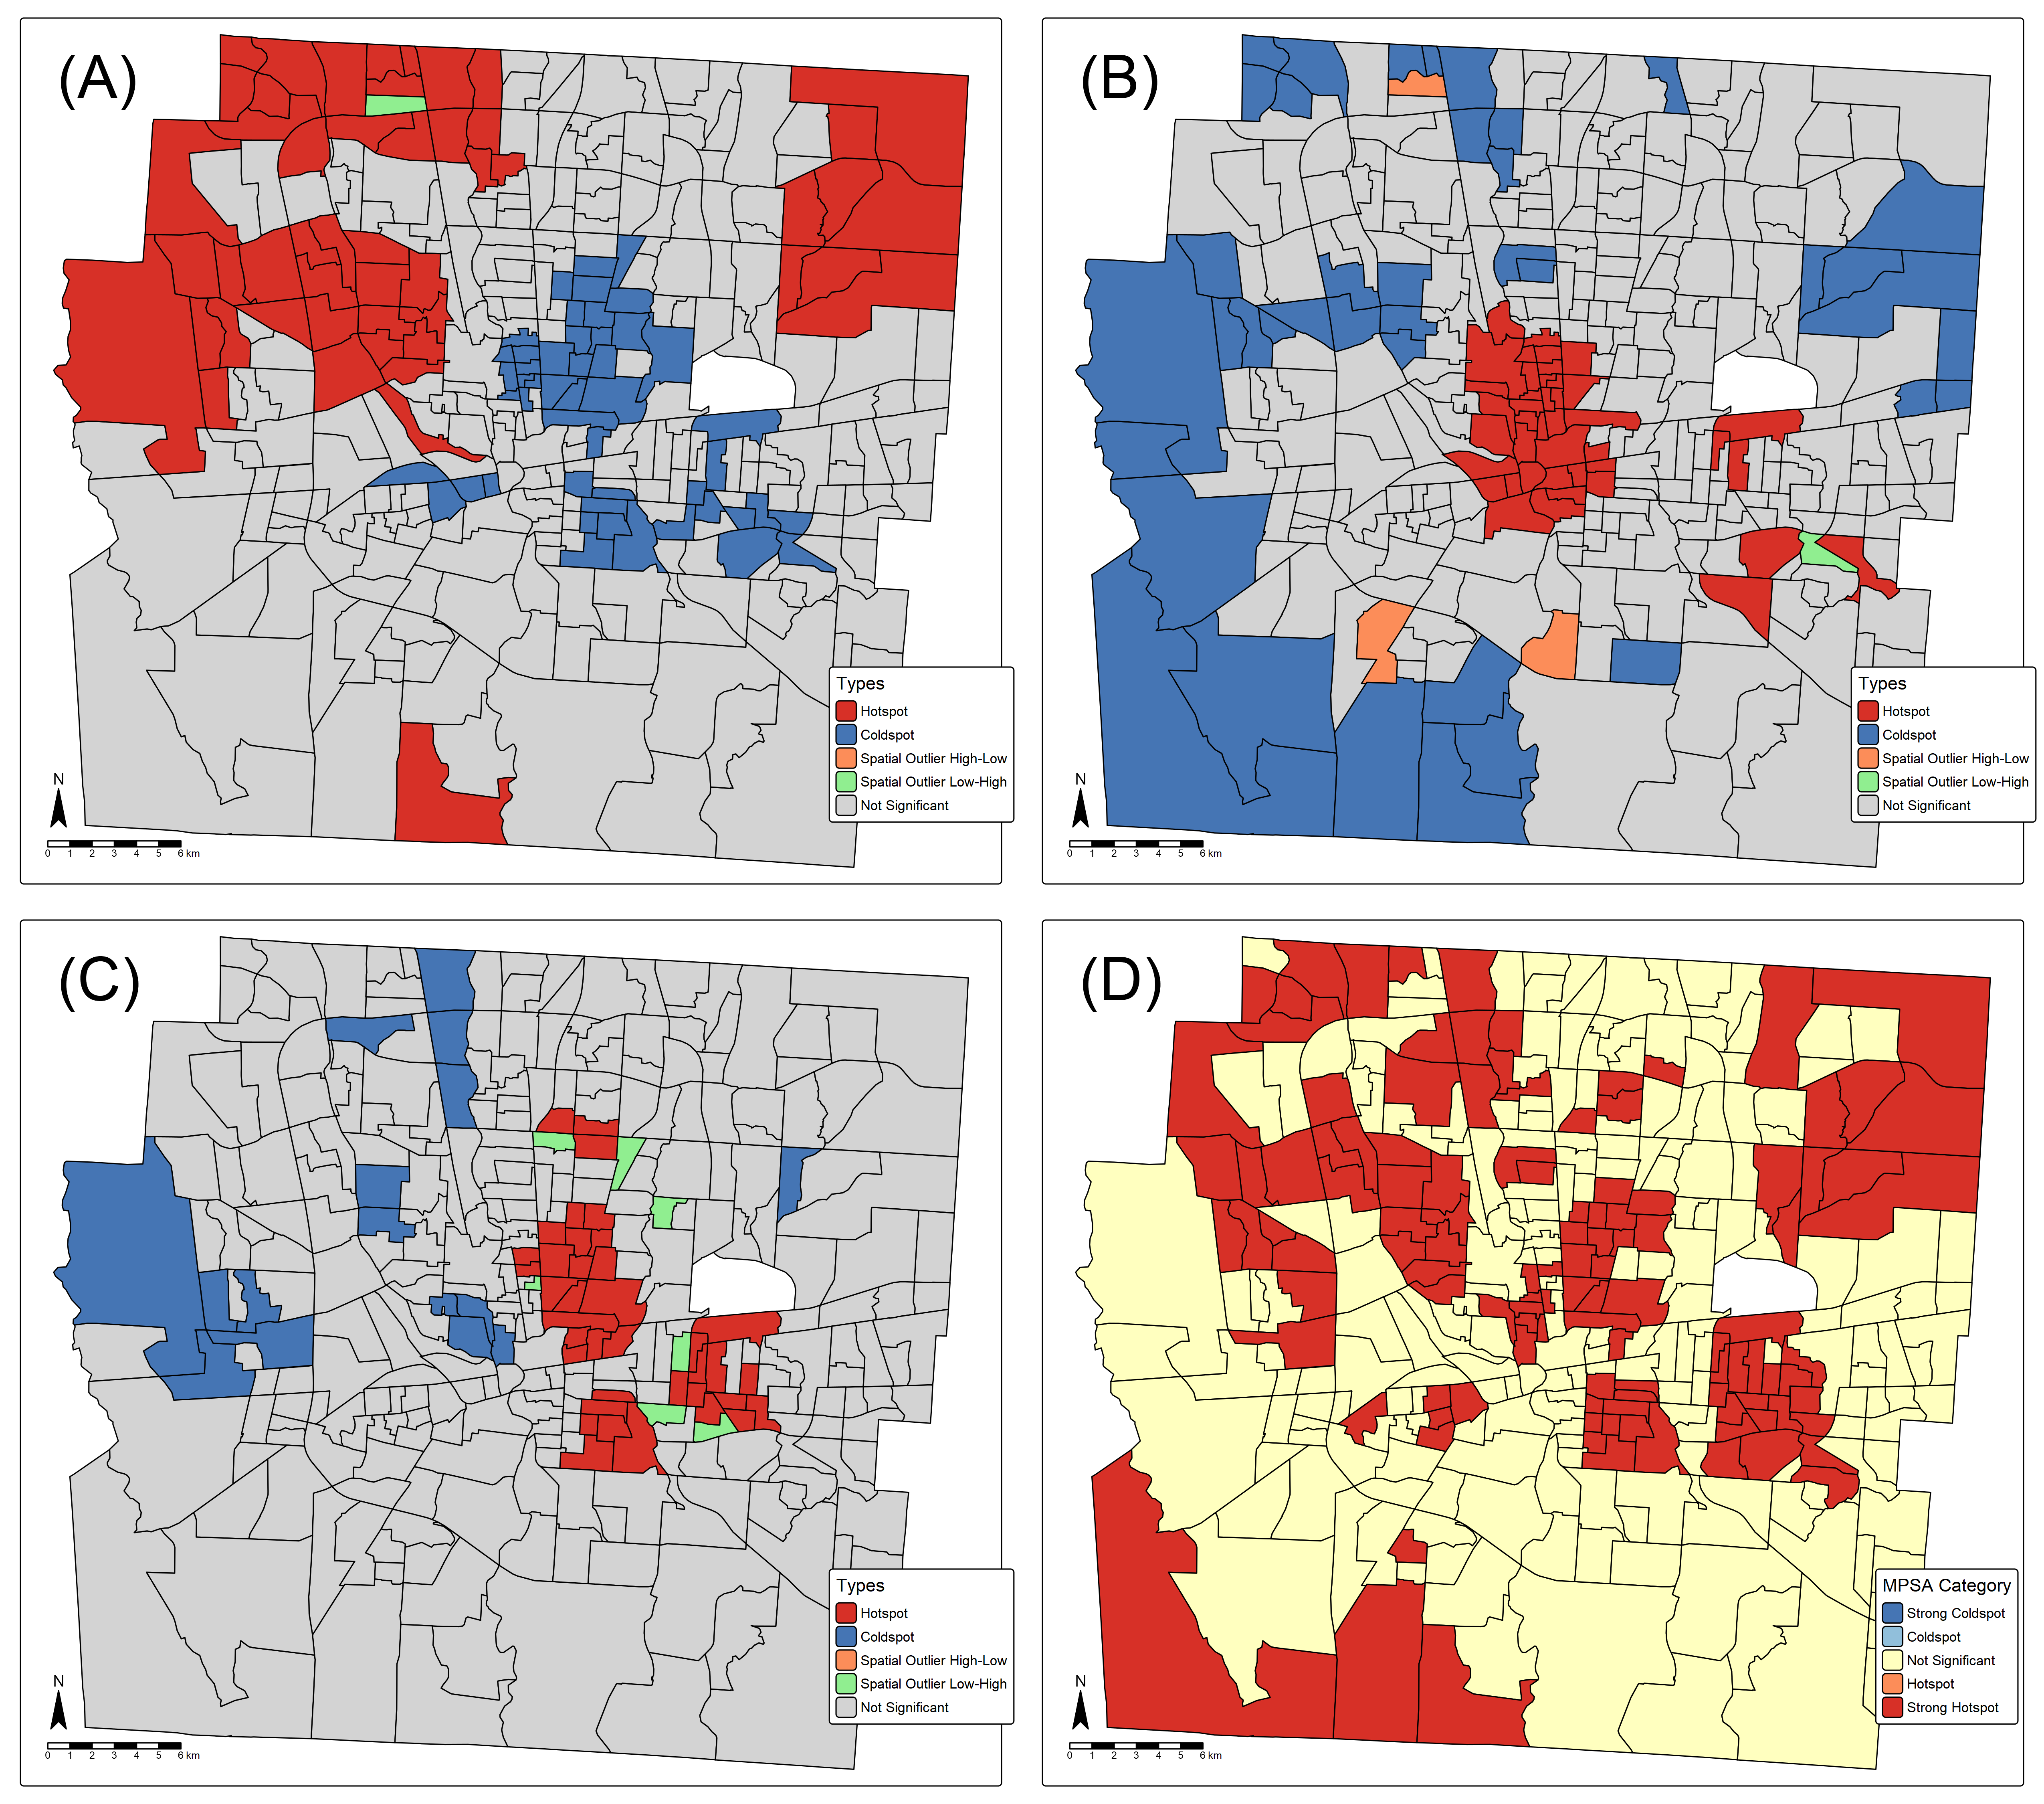
\includegraphics[width=0.8\textwidth]{output/robustness/data_description.png}
\caption{\small Local spatial association maps. (A), (B), and (C) represent the significance maps of local Moran’s I for median household income, renter-occupied housing(\%), and unemployment rate, respectively. (D) presents the local MPSA significance map, indicating clusters of spatially similar multivariate profiles. Colors denote statistically significant hotspots.}
\label{fig:data_description}
\end{figure}

\subsection{Stability of MPSA under Random Seed and Hyperparameter
Variation}\label{stability-of-mpsa-under-random-seed-and-hyperparameter-variation}

As previously described, the MPSA is a non-parametric statistic defined
based on random forests. Because the model training process involves
bootstrap sampling and random selection of predictor variables, a
certain level of randomness is inherently included in the computation.
Consequently, even when applied to the same dataset, MPSA values may
vary if the random seed is not fixed or if different hyperparameter
settings are used. To empirically assess the stability of MPSA under
such randomness and sensitivity to parameter settings, MPSA was computed
100 times without fixing the random seed while varying \emph{ntree}.
This procedure enabled the consistency of the statistic's distribution
under each tree count to be examined. The reliability of the statistic
was quantitatively analyzed by comparing and visualizing the mean and
variance of the MPSA values for each configuration. \vspace{1em}

\begin{table}[htb]
\centering
\caption{Mean, Standard Deviation, and Coefficient of Variation of MPSA Values by Number of Trees (\textit{ntree})}
\label{tab:mpsa_ntree_cv}
\begin{tabular}{cccc}
\toprule
\textit{ntree} & \textbf{Mean MPSA} & \textbf{Standard Deviation} & \textbf{Coefficient of Variation (CV)} \\
\midrule
50   & 0.033 & 0.0016  & 0.0480 \\
100  & 0.044 & 0.0017  & 0.0386 \\
500  & 0.058 & 0.0012  & 0.0204 \\
1000 & 0.061 & 0.0010   & 0.0161 \\
\bottomrule
\end{tabular}
\end{table}

\subsubsection{Global MPSA}\label{global-mpsa}

As shown in Table \ref{tab:mpsa_ntree_cv}, the mean MPSA values
increased with larger \emph{ntree} values, indicating improved stability
in capturing multivariate spatial structure as the ensemble size grows.
Notably, the standard deviation decreased as \emph{ntree} increased, and
the coefficient of variation (CV) declined from 0.0480 at \emph{ntree} =
50 to 0.0161 at \emph{ntree} = 1000, suggesting enhanced statistical
consistency with larger forests.

\begin{figure}[H]
\centering
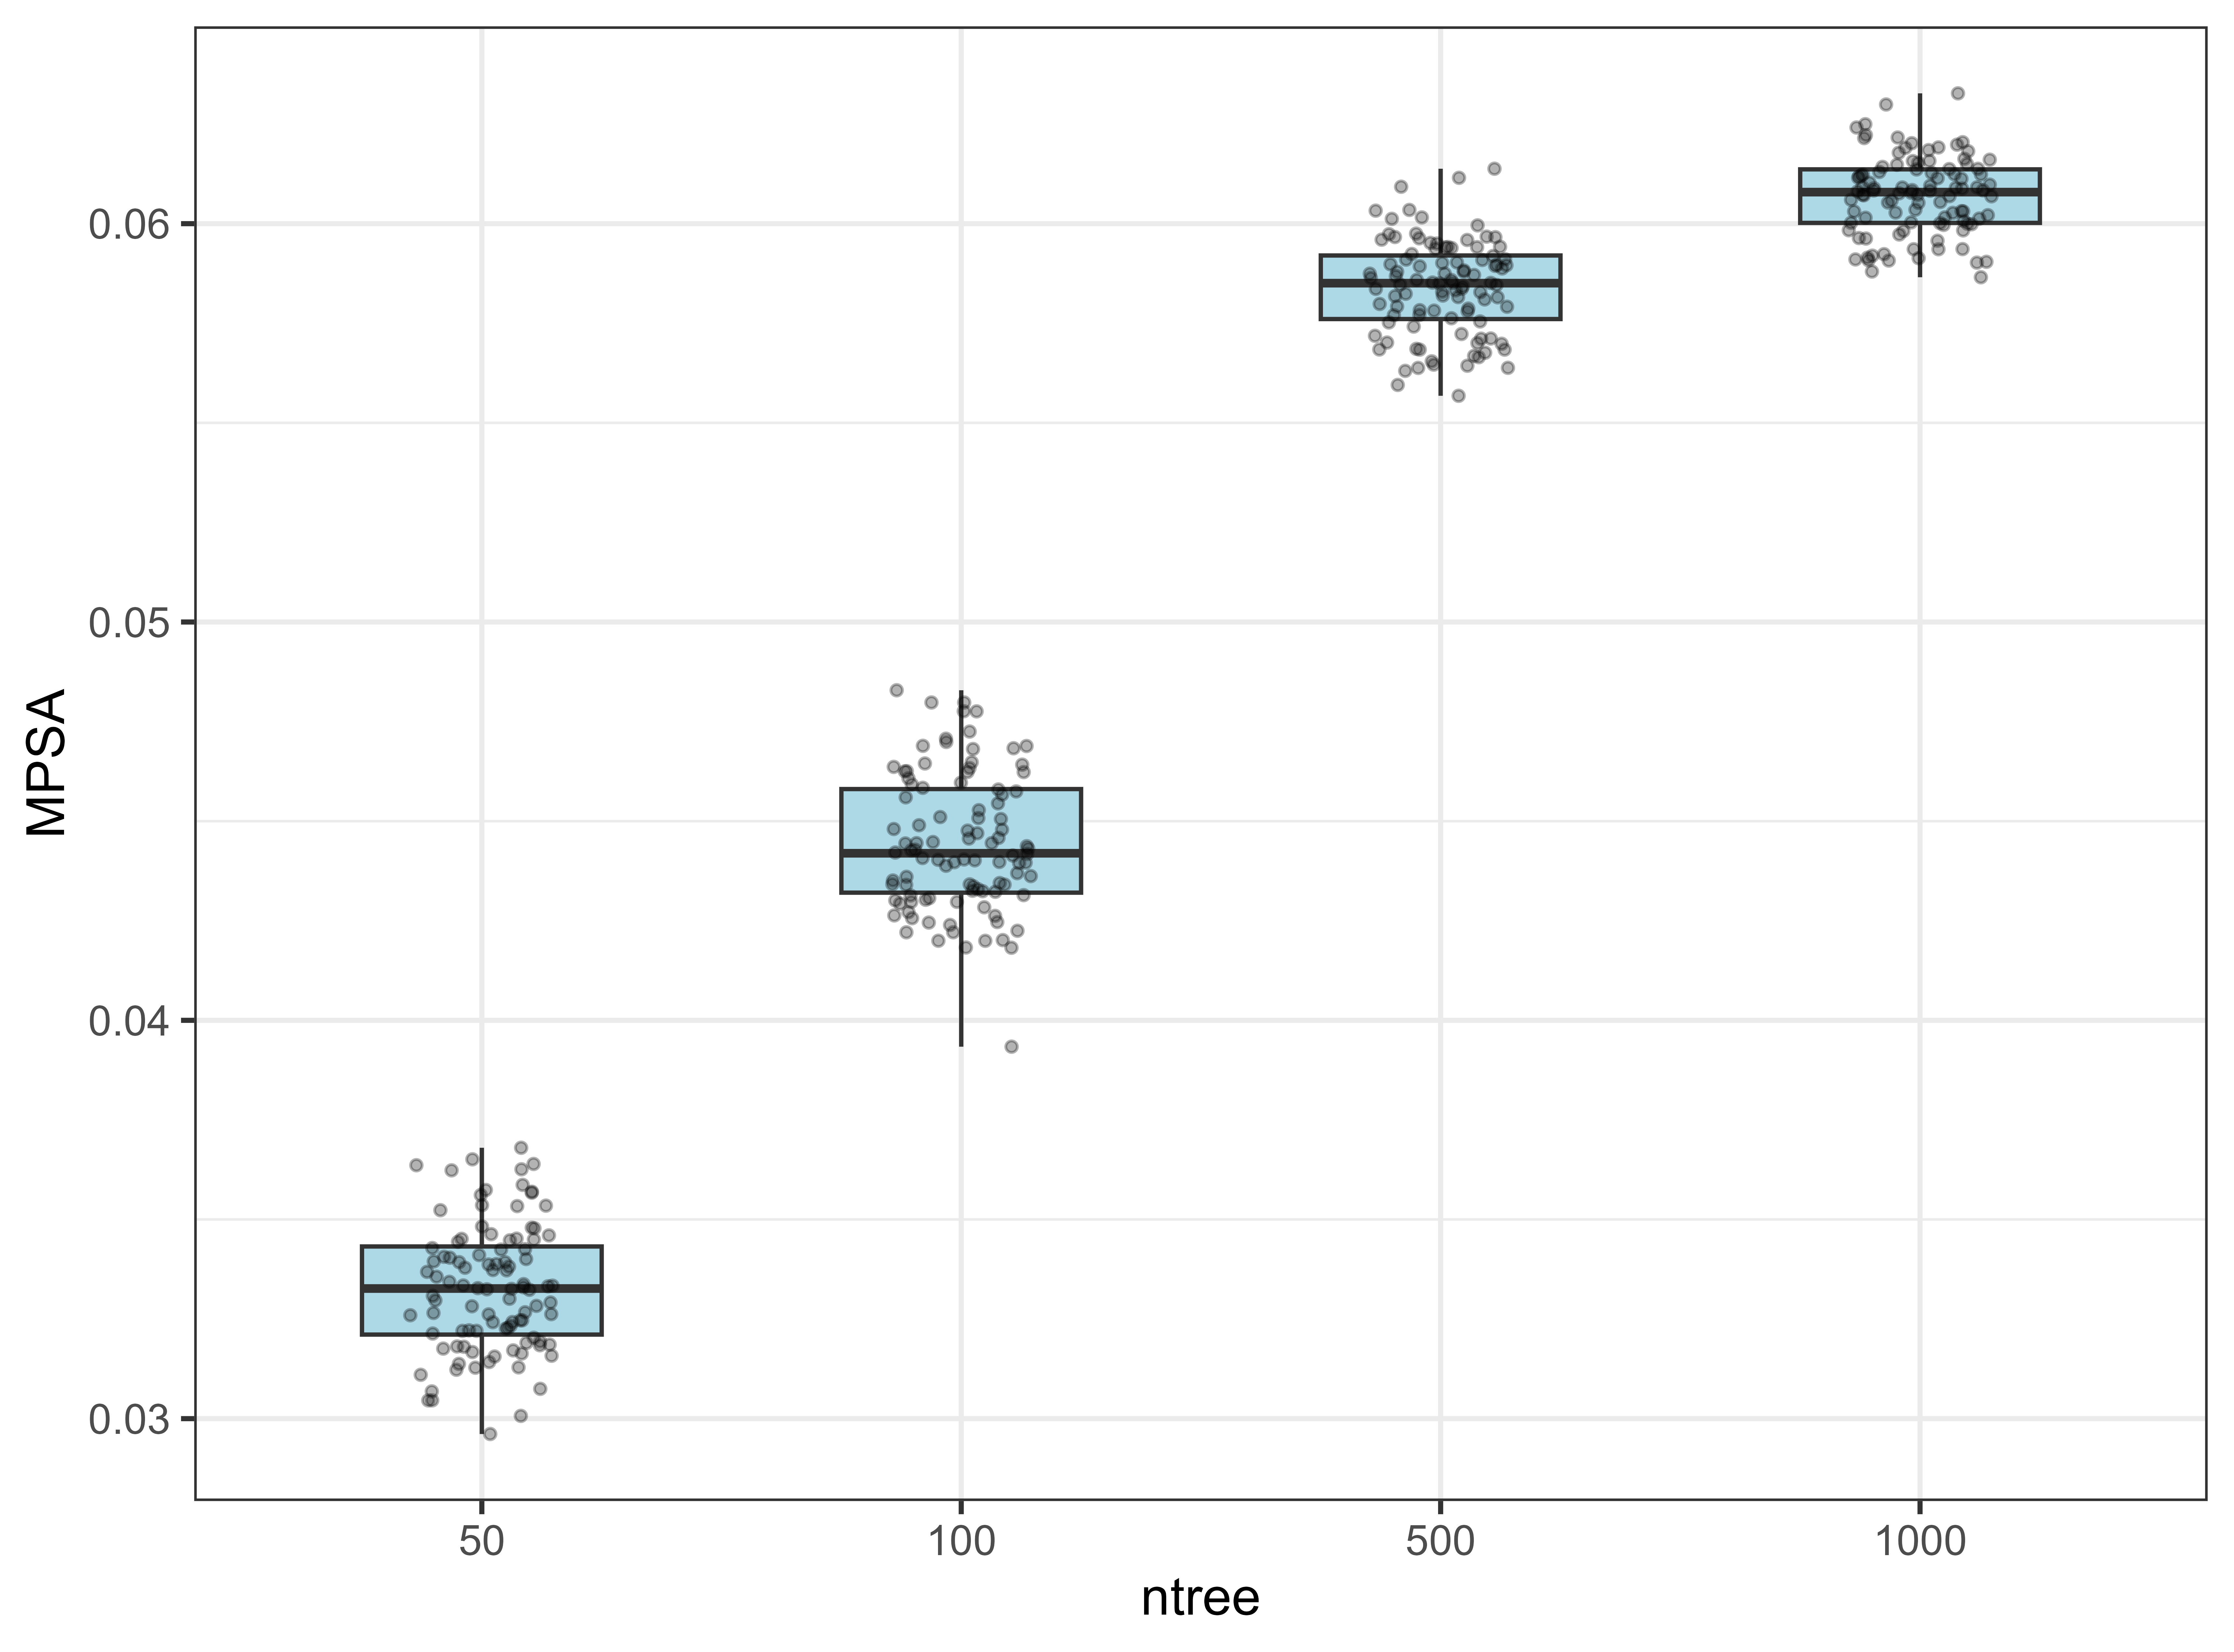
\includegraphics[width=0.95\textwidth]{output/robustness/global_mpsa_boxplot.png}
\caption{\small Distribution of MPSA values across different values of \textit{ntree}}
\label{fig:global_mpsa_boxplot}
\end{figure}

Figure \ref{fig:global_mpsa_boxplot} further visualizes the distribution
of MPSA values across different \emph{ntree} settings. The boxplots
clearly show that while the central tendency (median and mean) becomes
more stable with increasing \emph{ntree}, the variability around these
central values also contracts. In particular, the dispersion of MPSA
values is most pronounced at \emph{ntree} = 50, with the interquartile
range decreasing as the number of trees increases.

Importantly, however, even at lower values such as \emph{ntree} = 50 or
100, the standard deviation and coefficient of variation remain
sufficiently small (CV \textless{} 0.05), indicating that the MPSA
statistic exhibits a relatively high degree of stability across
repetitions. This implies that, depending on computational constraints,
a moderate number of trees may still be adequate to ensure reliable
results without substantial loss of robustness. Thus, the proposed MPSA
offers both statistical consistency and practical efficiency even under
limited \emph{ntree} sizes.

\subsubsection{Local MPSA}\label{local-mpsa}

For the local MPSA, we adopted the same procedure used for the global
statistic: without fixing the random seed, the local MPSA was computed
100 times for each of the tree counts set to 50, 100, 500, and 1000. For
each spatial unit, the mean and standard deviation of the resulting
local MPSA values were calculated, and the coefficient of variation (CV)
was subsequently derived. The ranges of CV for each \emph{ntree} are
summarized in Table \ref{tab:local_mpsa_cv_summary} and the spatial
distribution is presented in Figure \ref{fig:local_mpsa_cv}

\vspace{1em}

\begin{table}[htb]
\centering
\caption{Summary Statistics of Local MPSA Coefficient of Variation (CV) by \textit{ntree} Settings}
\label{tab:local_mpsa_cv_summary}
\begin{tabular}{lrrrrrr}
\toprule
\textit{ntree} & Min   & 1st Quartile & Median & Mean  & 3rd Quartile & Max   \\
\midrule
50   & 0.1436 & 0.2364 & 0.2691 & 0.2764 & 0.3090 & 0.5337 \\
100  & 0.1104 & 0.1685 & 0.1848 & 0.1899 & 0.2103 & 0.3162 \\
500  & 0.0493 & 0.0714 & 0.0802 & 0.0822 & 0.0909 & 0.1455 \\
1000 & 0.0342 & 0.0513 & 0.0576 & 0.0586 & 0.0659 & 0.1100 \\
\bottomrule
\end{tabular}
\end{table}
\begin{figure}[htb]
\centering
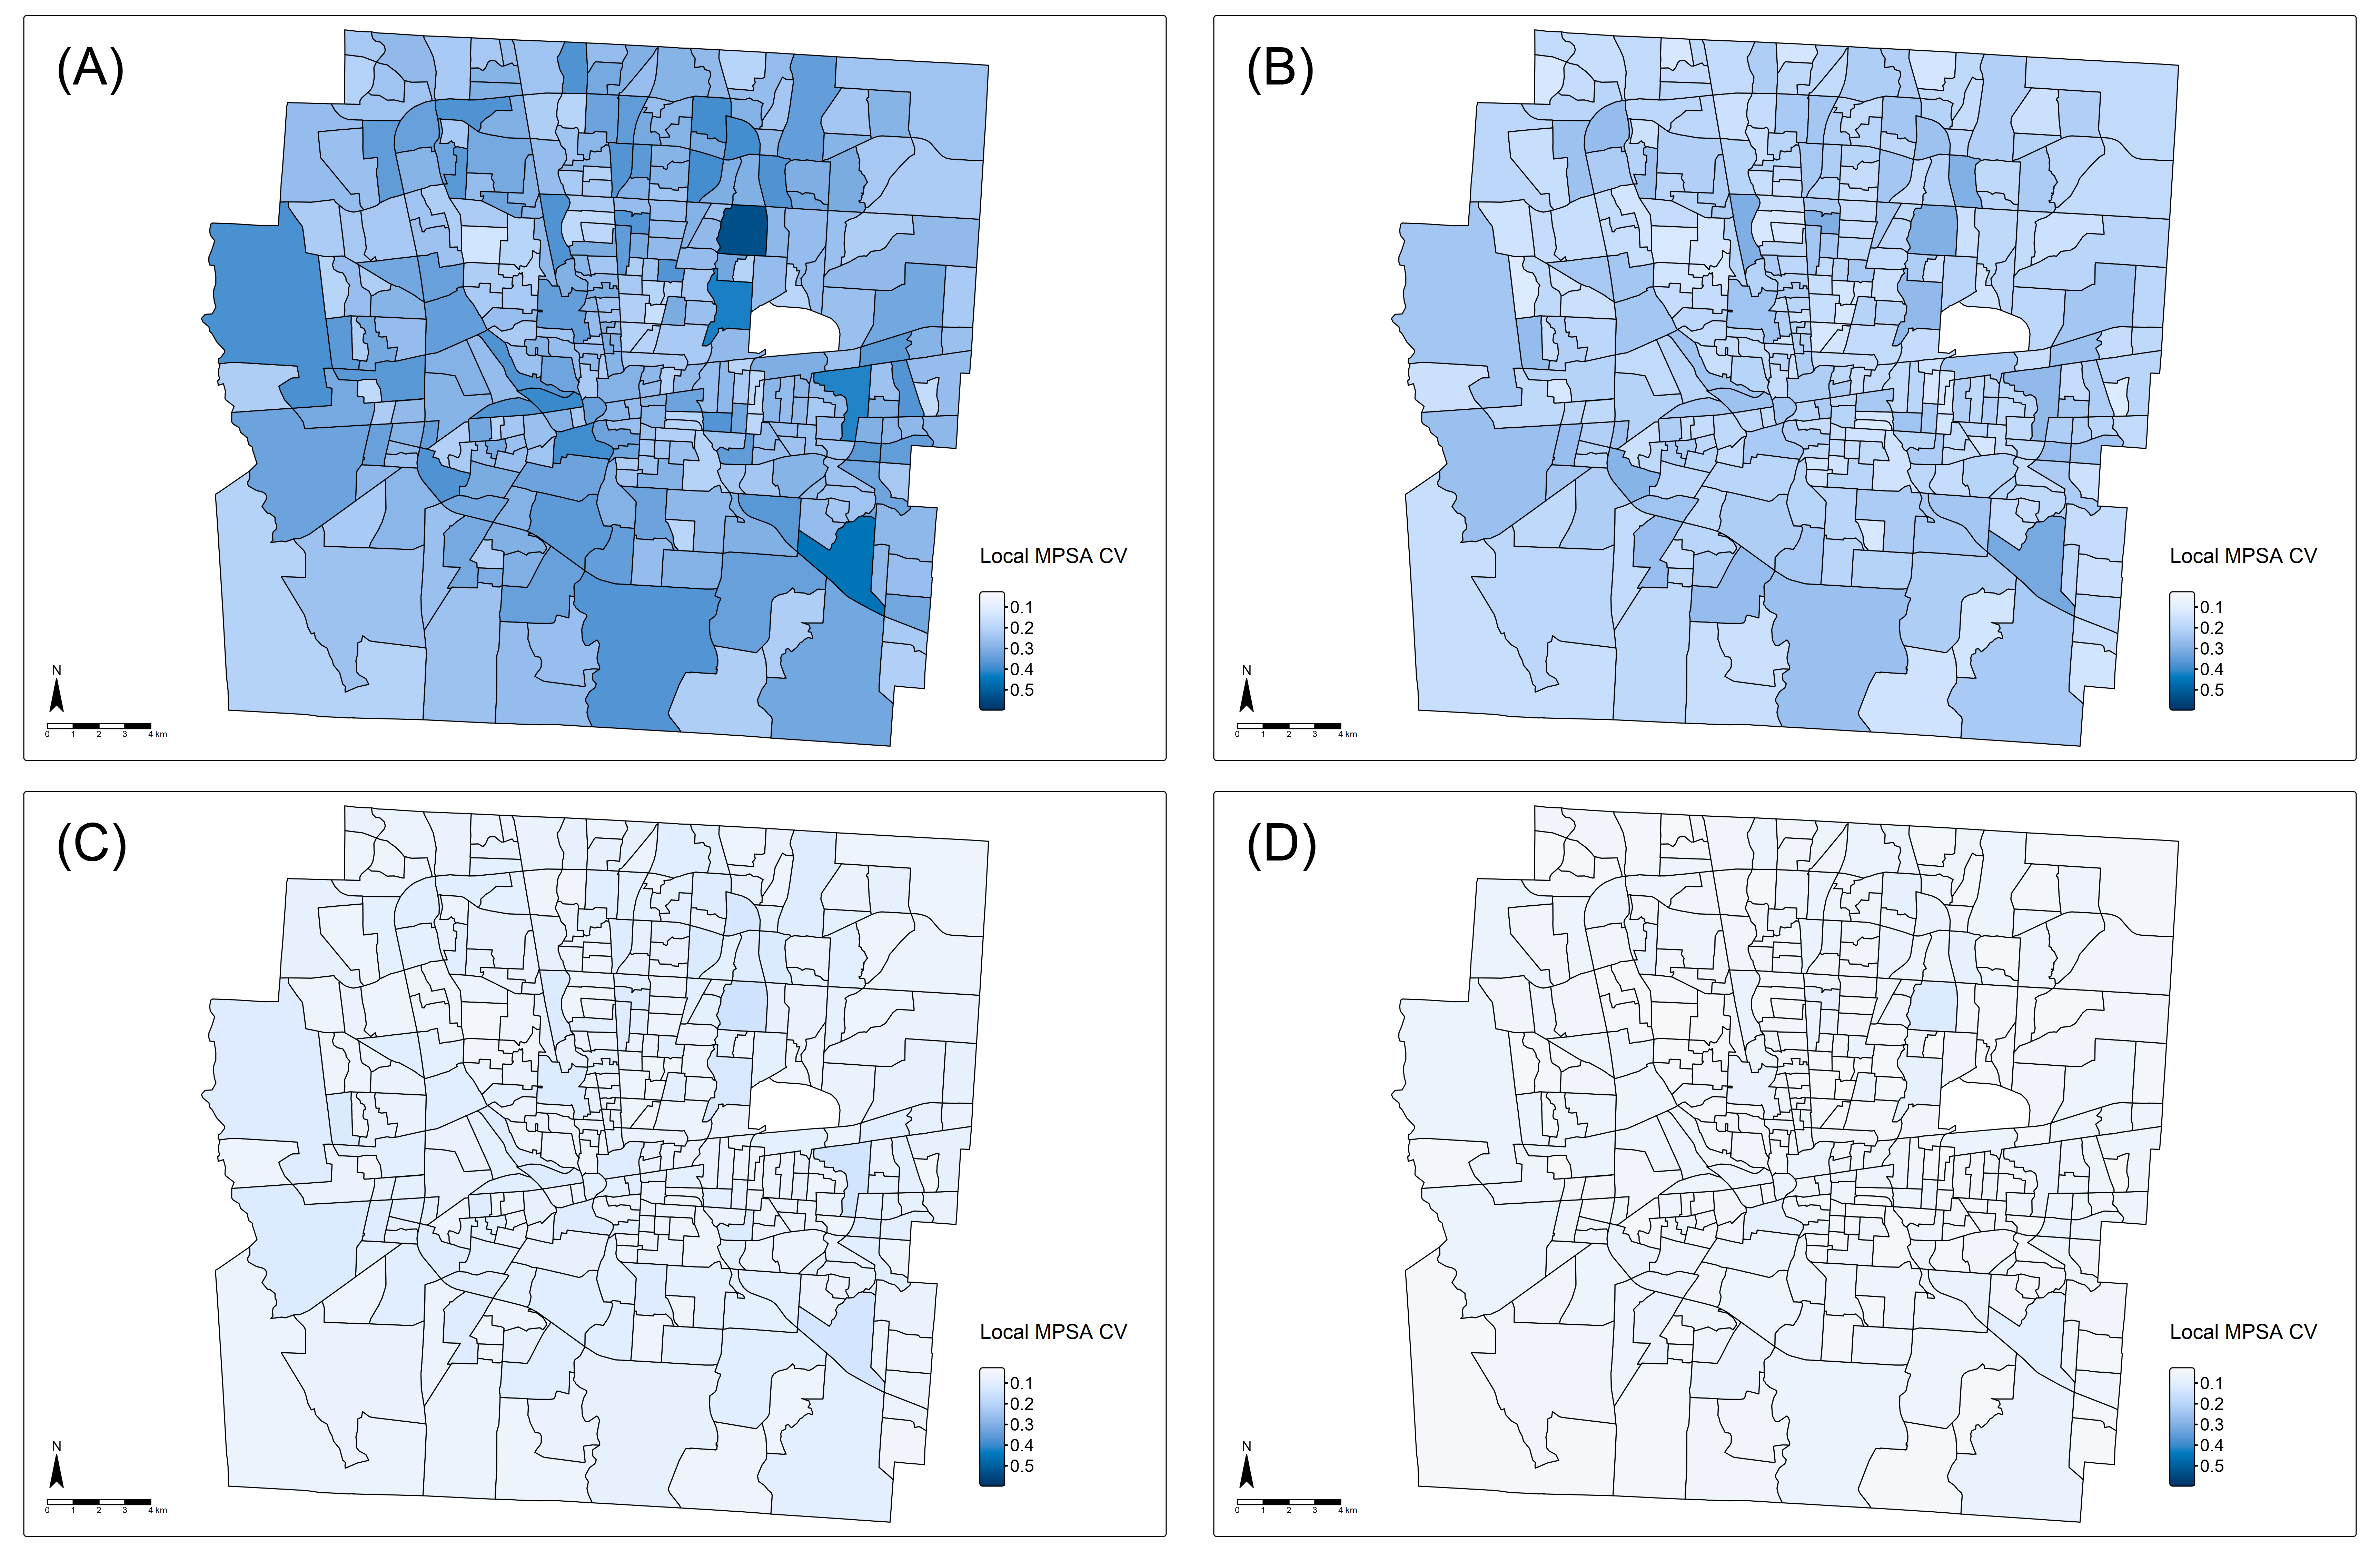
\includegraphics[width=0.95\textwidth]{output/robustness/local_mpsa_cv.png}
\caption{\small Spatial distribution of the coefficient of variation (CV) of local MPSA values across different numbers of trees in the random forest model.
(A) \textit{ntree} = 50 (B) \textit{ntree} = 100 (C) \textit{ntree} = 500 (D) \textit{ntree} = 1000.
The color scale indicates the relative magnitude of local instability (CV), with darker shades representing greater variability.
All four maps use a consistent legend range (0.1–0.6) for visual comparability.}
\label{fig:local_mpsa_cv}
\end{figure}

\section{Disscusion and Conclusion}\label{disscusion-and-conclusion}

\section*{Reference}\label{refs}
\addcontentsline{toc}{section}{Reference}

\phantomsection\label{refs}
\begin{CSLReferences}{1}{1}
\bibitem[\citeproctext]{ref-aggarwal2001}
Aggarwal, Charu C., Alexander Hinneburg, and Daniel A. Keim. 2001.
\emph{On the Surprising Behavior of Distance Metrics in High Dimensional
Space}. Edited by Jan Van den Bussche and Victor Vianu. Springer Berlin
Heidelberg.

\bibitem[\citeproctext]{ref-anselin1995}
Anselin, Luc. 1995. {``Local Indicators of Spatial
Association{\textemdash}LISA.''} \emph{Geographical Analysis} 27 (2):
93--115. \url{https://doi.org/10.1111/j.1538-4632.1995.tb00338.x}.

\bibitem[\citeproctext]{ref-anselin2019}
Anselin, Luc. 2019. {``A Local Indicator of Multivariate Spatial
Association: Extending Geary's {\emph{c}}.''} \emph{Geographical
Analysis} 51 (2): 133--50. \url{https://doi.org/10.1111/gean.12164}.

\bibitem[\citeproctext]{ref-benjamini1995}
Benjamini, Yoav, and Yosef Hochberg. 1995. {``Controlling the False
Discovery Rate: A Practical and Powerful Approach to Multiple
Testing.''} \emph{Journal of the Royal Statistical Society: Series B
(Methodological)} 57 (1): 289--300.

\bibitem[\citeproctext]{ref-beyer1999}
Beyer, Kevin, Jonathan Goldstein, Raghu Ramakrishnan, and Uri Shaft.
1999. \emph{When Is {``}Nearest Neighbor{''} Meaningful?} Edited by
Catriel Beeri and Peter Buneman. Springer Berlin Heidelberg.

\bibitem[\citeproctext]{ref-breiman2001}
Breiman, Leo. 2001. {``Random Forests.''} \emph{Machine Learning} 45
(1): 5--32.

\bibitem[\citeproctext]{ref-breiman2003}
Breiman, Leo. 2003. \emph{Manual on Setting up, Using, and Understanding
Random Forests V3.1}.

\bibitem[\citeproctext]{ref-geary1954}
Geary, R. C. 1954. {``The Contiguity Ratio and Statistical Mapping.''}
\emph{The Incorporated Statistician} 5 (3): 115--46.
\url{https://doi.org/10.2307/2986645}.

\bibitem[\citeproctext]{ref-kruber2019}
Kruber, Friedrich, Jonas Wurst, Eduardo Sánchez Morales, Samarjit
Chakraborty, and Michael Botsch. 2019. {``Unsupervised and Supervised
Learning with the Random Forest Algorithm for Traffic Scenario
Clustering and Classification.''} \emph{2019 IEEE Intelligent Vehicles
Symposium (IV)}, June, 2463--70.
\url{https://doi.org/10.1109/IVS.2019.8813994}.

\bibitem[\citeproctext]{ref-lee2012}
Lee, Monghyeon. 2012. {``Multivariate Spatial Cluster Analysis Using
Mahalanobis Distance.''} \emph{Journal of the Korean Cartographic
Association} 12 (2): 37--46.

\bibitem[\citeproctext]{ref-lee2001}
Lee, Sang-Il. 2001. {``Developing a Bivariate Spatial Association
Measure: An Integration of Pearson's r and Moran's I.''} \emph{Journal
of Geographical Systems} 3 (4): 369--85.
\url{https://doi.org/10.1007/s101090100064}.

\bibitem[\citeproctext]{ref-moran1950}
Moran, P. A. P. 1950. {``Notes on Continuous Stochastic Phenomena.''}
\emph{Biometrika} 37 (1/2): 17--23.
\url{https://doi.org/10.2307/2332142}.

\bibitem[\citeproctext]{ref-omar2022}
Omar, Zaturrawiah Ali, Mohd Aftar Abu Bakar, Zamira Hasanah Zamzuri, and
Noratiqah Mohd Ariff. 2022. {``Duplicate Detection Using Unsupervised
Random Forests: A Preliminary Analysis.''} \emph{2022 3rd International
Conference on Artificial Intelligence and Data Sciences (AiDAS)},
September, 66--71.
\url{https://doi.org/10.1109/AiDAS56890.2022.9918724}.

\bibitem[\citeproctext]{ref-peerbhay2015}
Peerbhay, Kabir Yunus, Onisimo Mutanga, and Riyad Ismail. 2015.
{``Random Forests Unsupervised Classification: The Detection and Mapping
of Solanum Mauritianum Infestations in Plantation Forestry Using
Hyperspectral Data.''} \emph{IEEE Journal of Selected Topics in Applied
Earth Observations and Remote Sensing} 8 (6): 3107--22.
\url{https://doi.org/10.1109/JSTARS.2015.2396577}.

\bibitem[\citeproctext]{ref-peerbhay2016}
Peerbhay, Kabir Yunus, Onisimo Mutanga, Romano Lottering, and Riyad
Ismail. 2016. {``Unsupervised Anomaly Weed Detection in Riparian Forest
Areas Using Hyperspectral Data and LiDAR.''} \emph{2016 8th Workshop on
Hyperspectral Image and Signal Processing: Evolution in Remote Sensing
(WHISPERS)}, August, 1--5.
\url{https://doi.org/10.1109/WHISPERS.2016.8071797}.

\bibitem[\citeproctext]{ref-shi2006}
Shi, Tao, and Steve Horvath. 2006. {``Unsupervised Learning with Random
Forest Predictors.''} \emph{Journal of Computational and Graphical
Statistics} 15 (1): 118--38.

\bibitem[\citeproctext]{ref-wartenberg1985}
Wartenberg, Daniel. 1985. {``Multivariate Spatial Correlation: A Method
for Exploratory Geographical Analysis.''} \emph{Geographical Analysis}
17 (4): 263--83.
\url{https://doi.org/10.1111/j.1538-4632.1985.tb00849.x}.

\bibitem[\citeproctext]{ref-wu2007}
Wu, Sean H., Benjamin N. Lee, Li-C. Wang, and Magdy S. Abadir. 2007.
{``Statistical Analysis and Optimization of Parametric Delay Test.''}
\emph{2007 IEEE International Test Conference}, October, 1--10.
\url{https://doi.org/10.1109/TEST.2007.4437626}.

\bibitem[\citeproctext]{ref-zhang2008}
Zhang, Jiong, Mohammad Zulkernine, and Anwar Haque. 2008.
{``Random-Forests-Based Network Intrusion Detection Systems.''}
\emph{IEEE Transactions on Systems, Man, and Cybernetics, Part C
(Applications and Reviews)} 38 (5): 649--59.
\url{https://doi.org/10.1109/TSMCC.2008.923876}.

\end{CSLReferences}



\end{document}
